\documentclass{article}

% Recommended, but optional, packages for figures and better typesetting:
\usepackage{microtype}
\usepackage{graphicx}
% \usepackage{subfigure}
\usepackage{caption}
\usepackage{subcaption}
\usepackage{booktabs} % for professional tables
\usepackage{kotex} %korean patch

% hyperref makes hyperlinks in the resulting PDF.
% If your build breaks (sometimes temporarily if a hyperlink spans a page)
% please comment out the following usepackage line and replace
% \usepackage{icml2019} with \usepackage[nohyperref]{icml2019} above.
\usepackage{hyperref}

% Attempt to make hyperref and algorithmic work together better:
\newcommand{\theHalgorithm}{\arabic{algorithm}}

% Use the following line for the initial blind version submitted for review:
%\usepackage{icml2019}

% If accepted, instead use the following line for the camera-ready submission:
\usepackage[accepted]{icml2019}

% The \icmltitle you define below is probably too long as a header.
% Therefore, a short form for the running title is supplied here:
\icmltitlerunning{COSE474-2023F: Final Project Proposal}

\begin{document}

\twocolumn[
\icmltitle{COSE474-2021F: Final Project Proposal \\
           optimizer 가능성 탐구}

% It is OKAY to include author information, even for blind
% submissions: the style file will automatically remove it for you
% unless you've provided the [accepted] option to the icml2019
% package.

% List of affiliations: The first argument should be a (short)
% identifier you will use later to specify author affiliations
% Academic affiliations should list Department, University, City, Region, Country
% Industry affiliations should list Company, City, Region, Country

% You can specify symbols, otherwise they are numbered in order.
% Ideally, you should not use this facility. Affiliations will be numbered
% in order of appearance and this is the preferred way.
\icmlsetsymbol{equal}{*}

\begin{icmlauthorlist}
\icmlauthor{2019320138 김규진}{}
\end{icmlauthorlist}

%\icmlaffiliation{ku}{Department of Computer Science \& Engineering, Korea University, Seoul, Korea}


%\icmlcorrespondingauthor{the}{myemail@korea.ac.kr}
%\icmlcorrespondingauthor{Eee Pppp}{ep@eden.co.uk}

% You may provide any keywords that you
% find helpful for describing your paper; these are used to populate
% the "keywords" metadata in the PDF but will not be shown in the document
\icmlkeywords{Machine Learning, ICML}

\vskip 0.3in
]

% this must go after the closing bracket ] following \twocolumn[ ...

% This command actually creates the footnote in the first column
% listing the affiliations and the copyright notice.
% The command takes one argument, which is text to display at the start of the footnote.
% The \icmlEqualContribution command is standard text for equal contribution.
% Remove it (just {}) if you do not need this facility.

%\printAffiliationsAndNotice{}  % leave blank if no need to mention equal contribution
%\printAffiliationsAndNotice{\icmlEqualContribution} % otherwise use the standard text.

%\begin{abstract}
%This document provides a basic paper template and submission guidelines.
%Abstracts must be a single paragraph, ideally between 4--6 sentences long.
%Gross violations will trigger corrections at the camera-ready phase.
%\end{abstract}

\section{Introduction}
딥러닝 과정에서 설정하고 연결해줘야 할 모듈들로는 activation function, normalize, regularize 등 기본적인 부분에서조차 다양한 방식이 사용되고 있으며, 학습하는 모델에 따라 어떤 것을 활용해야 할지 설정해야 최적의 결과를 얻을 수 있다. 이중 적절한 optimizer을 정하는 것도 결과에 영향을 주는 주요한 부분으로 알려져 있다. Optimizer를 잘 선택한다면 연산량을 획기적으로 줄일 수 있기 때문에 결과가 나오기까지 기다려야 하는 시간을 최소화할 수 있고, 결과값 또한 더 최적값을 이끌어낼 수 있다. Momentum은 이름에서 볼 수 있듯 관성을 활용한 방식인데, 이처럼 optimizer에는 각각 현실에서 어떤 개념을 가지고 optimizer을 구현하고 있다. 그래서 이번 연구에서 또한 직접 철학적인 개념을 활용해 여러 optimizer을 고안해 적용해보고자 했다.
Base가 되는 모델로는 momentum을 이용했다. 관성을 이용하는 가장 기본적인 모델이기도 하며, 다양한 optimizer가 momentum에서 파생해 만들어졌기 때문에 선택하게 되었다. 또, learning rate를 연산과정에 넣어 따로 scheduling을 진행하는 기본적인 의례와는 달리, learning rate를 optimizer에서 고려하도록 설계해 차별점을 주었다.\\
새로운 개념의 optimizer들을 활용한다면 나머지 같은 모듈들을 활용한다 하더라도 작은 learning rate를 이용하더라도 더 적은 epoch를 이용해도 결과를 더 빠르게 도출해낼 수 있을 것이라고 예상하고 진행했다.\\
하지만 두 가지 개념을 이용해 만든 두 가지 optimizer은 모두 아쉽게도 유의미한 연산 속도 차이를 보여주지 못했다. 하지만, 이를 통해 왜 learning rate를 learning scheduler를 이용해 작업을 하는 것이 나은지 알게 되었고, 각 기능마다 의존성을 떨어뜨리는 것이 작업 능률이 좋다는 것을 알 수 있었다.

\section{Methods}
여기서는 optimizer을 만드는 데 있어 새로운 개념을 도입한 두 가지 새로운 optimizer을 이용한다. 이 두 가지는 learning rate를 결과값을 향한 중력 방식의 가속도의 강도라는 개념을 도입한 gravity optimizer와, momentum이 가리키는 방향과 진행방향이 다르다면 급격한 가중치를 주어 방향을 전환시키는 cosine optimizer을 소개한다.\\
1. gravity optimizer\\
첫 번째 소개할 방식은 gravity optimizer이다. 이는 기본적인 weight의 방향 말고, 결과값을 향한 가속도를 lr의 크기로 설정한다. 이를 통해 벡터가 클수록 더 강한 속도로 학습되고 있음을 보정한다. Algorithm~\ref{alg:gravity} 이 그 의사코드 형태를 보여준다.

\begin{algorithm}[tb]
   \caption{Gravity Optimizer}
   \label{alg:gravity}
\begin{algorithmic}
   \STATE {\bfseries Input:} parameter matrix array $params$, gradient matrix array $grad$, learning rate $lr$
   \STATE S=0
   \REPEAT
   \STATE for param in params
   \FOR {$param$ {\bfseries in} $params$}
   \STATE $ S += \sum{grad^2}$
   \ENDFOR
   \FOR {$param$ {\bfseries in} $params$}
   \STATE $define k as \sum{\sqrt{\frac{1}{lr^2}+\frac{1}{grad^2}}}$
   \STATE $param-=\frac{grad}{k}$
   \ENDFOR
   \UNTIL{backpropagations are finished}
\end{algorithmic}
\end{algorithm}

2. cosine optimizer\\
두 번째 소개할 방식은 cosine optimizer이다. 이는 현재 진행방향이 이번에 받은 가속도와 방향이 많이 다를수록, 더 확실하게 이번 가속도를 많이 반영하는 방식이다. Algorithm~\ref{alg:cosine} 가 의사코드 형태를 보인다.

\begin{algorithm}[tb]
   \caption{Cosine Optimizer}
   \label{alg:cosine}
\begin{algorithmic}
   \STATE {\bfseries Input:} parameter matrix array $params$, gradient matrix array $grad$, saver matrix array $m$, cosine value matrix array $cosine$, cosine constant $C$, learning rate $lr$
   \REPEAT
   \FOR {$param$ {\bfseries in} $params$}
   \FOR {$\vec{m}, \vec{g}, \vec{cos}$ {\bfseries in} $m, gradient, cosine$}
   \STATE $cos\theta=\frac{\vec{m}\cdot\vec{g}}{||m||\cdot||g||}$
   \STATE $\vec{cos}=cos\theta\cdot\vec{1}$
   \ENDFOR
   \STATE $m=C \frac{cosine}{2}m+lr\cdot gradient$
   \STATE $param-=m$
   \ENDFOR
   \UNTIL{backpropagations are finished}
\end{algorithmic}
\end{algorithm}

% 수식적으로 왜 그렇게 했는지 설명이 없음! 추가 필요

두가지 방식이 모두 효과적인 향상을 불러일으키지 못하더라도 optimizer을 실제로 구현해보며 optmizer에 대한 개인적 이해를 높일 수 있고, optimizer가 요구하는 사항이 어떤 것이 있는지 더 자세하게 알아볼 수 있을 것이다.
plateau현상과 zigzag가 가장 optimizer의 과제이다. 이를 위해 Momentum방식을 이용했지만, 이는 zigzag 문제를 해결해주지 못했기에 adaptive방식과 혼합된 adam이 주로 사용되는 추세이다. nesterov momentum 방식은 비용에 비해 성능 향상이 적었다고 한다. 이에 많은 optimizer들 중 momentum optimizer을 이용한 결과와 비교하여 성능향상이 실제로 일어났는지 비교하고자 한다.

\section{Experiments}
% - Dataset
데이터셋은 튜토리얼에서 진행한 옷을 이용한 dataset을 이용한다.
% - Computing resource (CPU,GPU, OS, pytorch etc.)
computing resource는 dataset의 규모가 크지 않기에 CPU를 이용한다. windows 10 환경에서 실행했으며, pytorch를 활용해 코드를 작성한다.
% - Experimental design/setup
setup으로 python 3.10.4를 이용했다. ipynb로 작성되었다.
% - Quantitative results / comparison with baselines, SOTA
SOTA는 momentum으로 실행했을 때의 결과를 momentum으로 잡는다.
결과: 거의 변하지 않음...ㅜㅜ
다양한 learning rate 하에서 실행했지만, 큰 소득은 얻을 수 없었음
% - Figures (plots)/Tables and their analysis
결과 예시 사진 loss and accuracy. 여기서 img파일 안에 있는 사진 파일들을 활용한다.
\begin{figure}
   \centering
   \begin{subfigure}{0.3\columnwidth}
      \centering
      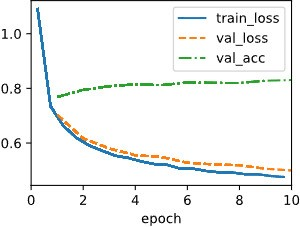
\includegraphics[width=\columnwidth]{img/lr0.1 sgd.jpg}
      \caption{sgd}
   \end{subfigure}
   \hfill
   \begin{subfigure}[b]{0.3\columnwidth}
      \centering
      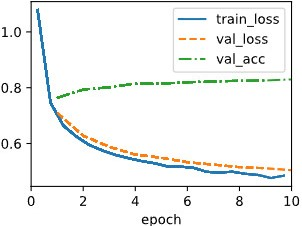
\includegraphics[width=\columnwidth]{img/lr0.1 gravity.jpg}
      \caption{gravity}
   \end{subfigure}
   \hfill
   \begin{subfigure}[b]{0.3\columnwidth}
      \centering
      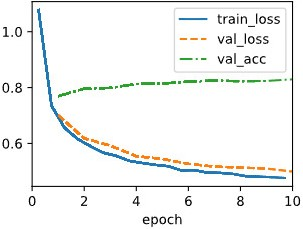
\includegraphics[width=\columnwidth]{img/lr0.1 cosine.jpg}
      \caption{cosine}
   \end{subfigure}
   \caption{lr=0.1}
      \label{lr-0.1}
\end{figure}

\begin{figure}[ht]
\vskip 0.2in
\begin{center}\centering
\begin{subfigure}[b]{0.3\columnwidth}\centering
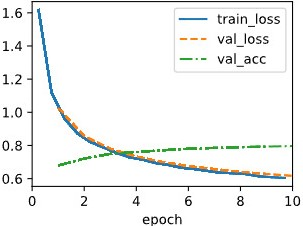
\includegraphics[width=\columnwidth]{img/lr0.01 sgd.jpg}
\end{subfigure}
\hfill
\begin{subfigure}[b]{0.3\columnwidth}\centering
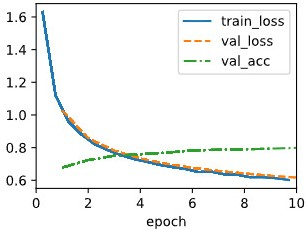
\includegraphics[width=\columnwidth]{img/lr0.01 gravity.jpg}
\end{subfigure}
\hfill
\begin{subfigure}[b]{0.3\columnwidth}\centering
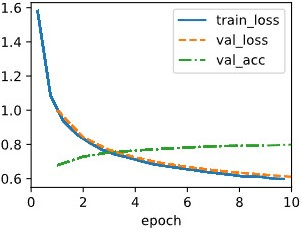
\includegraphics[width=\columnwidth]{img/lr0.01 cosine0.1.jpg}
\end{subfigure}
\hfill
\begin{subfigure}[b]{0.3\columnwidth}\centering
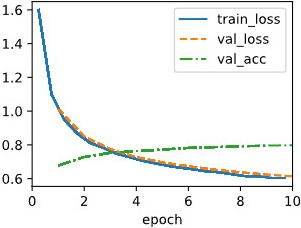
\includegraphics[width=\columnwidth]{img/lr0.01 cosine0.05.jpg}
\end{subfigure}
\hfill
\begin{subfigure}[b]{0.3\columnwidth}\centering
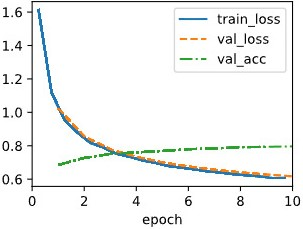
\includegraphics[width=\columnwidth]{img/lr0.01 cosine0.01.jpg}
\end{subfigure}
\caption{lr=0.01}
\label{lr-0.01}
\end{center}
\vskip -0.2in
\end{figure}

\begin{figure}[ht]
\vskip 0.2in
\begin{center}\centering
\begin{subfigure}[b]{0.3\columnwidth}\centering
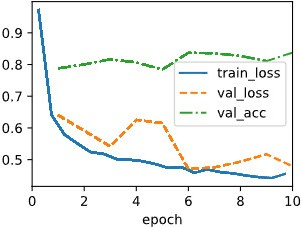
\includegraphics[width=\columnwidth]{img/lr0.2 sgd.jpg}
\end{subfigure}
\hfill
\begin{subfigure}[b]{0.3\columnwidth}\centering
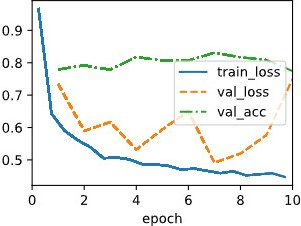
\includegraphics[width=\columnwidth]{img/lr0.2 gravity.jpg}
\end{subfigure}
\hfill
\begin{subfigure}[b]{0.3\columnwidth}\centering
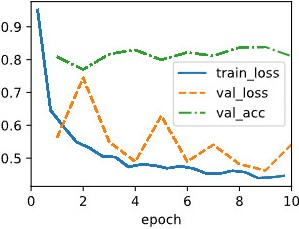
\includegraphics[width=\columnwidth]{img/lr0.2 cosine0.1.jpg}
\end{subfigure}
\hfill
\begin{subfigure}[b]{0.3\columnwidth}\centering
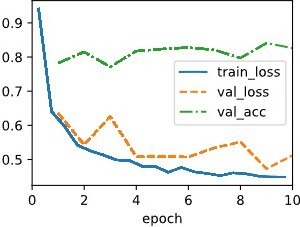
\includegraphics[width=\columnwidth]{img/lr0.2 cosine0.05.jpg}
\end{subfigure}
\hfill
\begin{subfigure}[b]{0.3\columnwidth}\centering
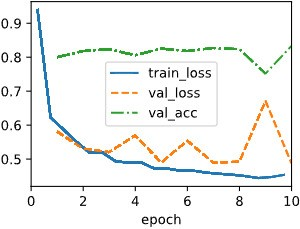
\includegraphics[width=\columnwidth]{img/lr0.2 cosine0.01.jpg}
\end{subfigure}
\caption{lr=0.2}
\label{lr-0.2}
\end{center}
\vskip -0.2in
\end{figure}
% - Discussion why the proposed method is successful or unsuccessful 
이게 왜 실패했는가? 너무 복잡하고, learning rate를 넣어서 게산한다고 해서 gradient가 드라마틱하게 달라지는 것이 아닌 것 같음. 그럼에도 미세한 차이가 보이는 것으로 보아 dataset이 너무 작아서 차이를 비교하기 어려운 수준이 아니었나 라는 예상이 됨.

% Improved adam optimizer\cite{ImpAdam}에 따르면 adam에 learning rate의 모멘텀을 적용하는 방법에 대해 고민한 내용이 있다. 다양한 optimizer 관련 논문이 작성되지만 선호되는 종류에 대해서만 다룰 뿐, learning rate를 선형적이지 않게 활용하는 방법은 찾을 수 없었다. cosine 역시 SGDR\cite{SGDR}에서 cosine 파동을 이용해 스케줄링을 하는 방법에대해선 연구하고 있지만, momentum과 gradient의 각도를 이용한 방법은 나오지 않고 있다.

\section{Future direction}
다음에는 다른 데이터셋을 활용해 훨씬 대규모의 데이터를 처리해 봐야할 것이다. epoch가 100은 되는 것을 해봐야하지 않을까?
classification을 활용하는 것은 그대로 가는 것이 좋을 것 같다.

\bibliography{example_paper}
\bibliographystyle{icml2019}
\clearpage



\end{document}
